% Standalone TikZ fragment for \input into the paper body.
% Assumes the document preamble already loads tikz and amsmath.
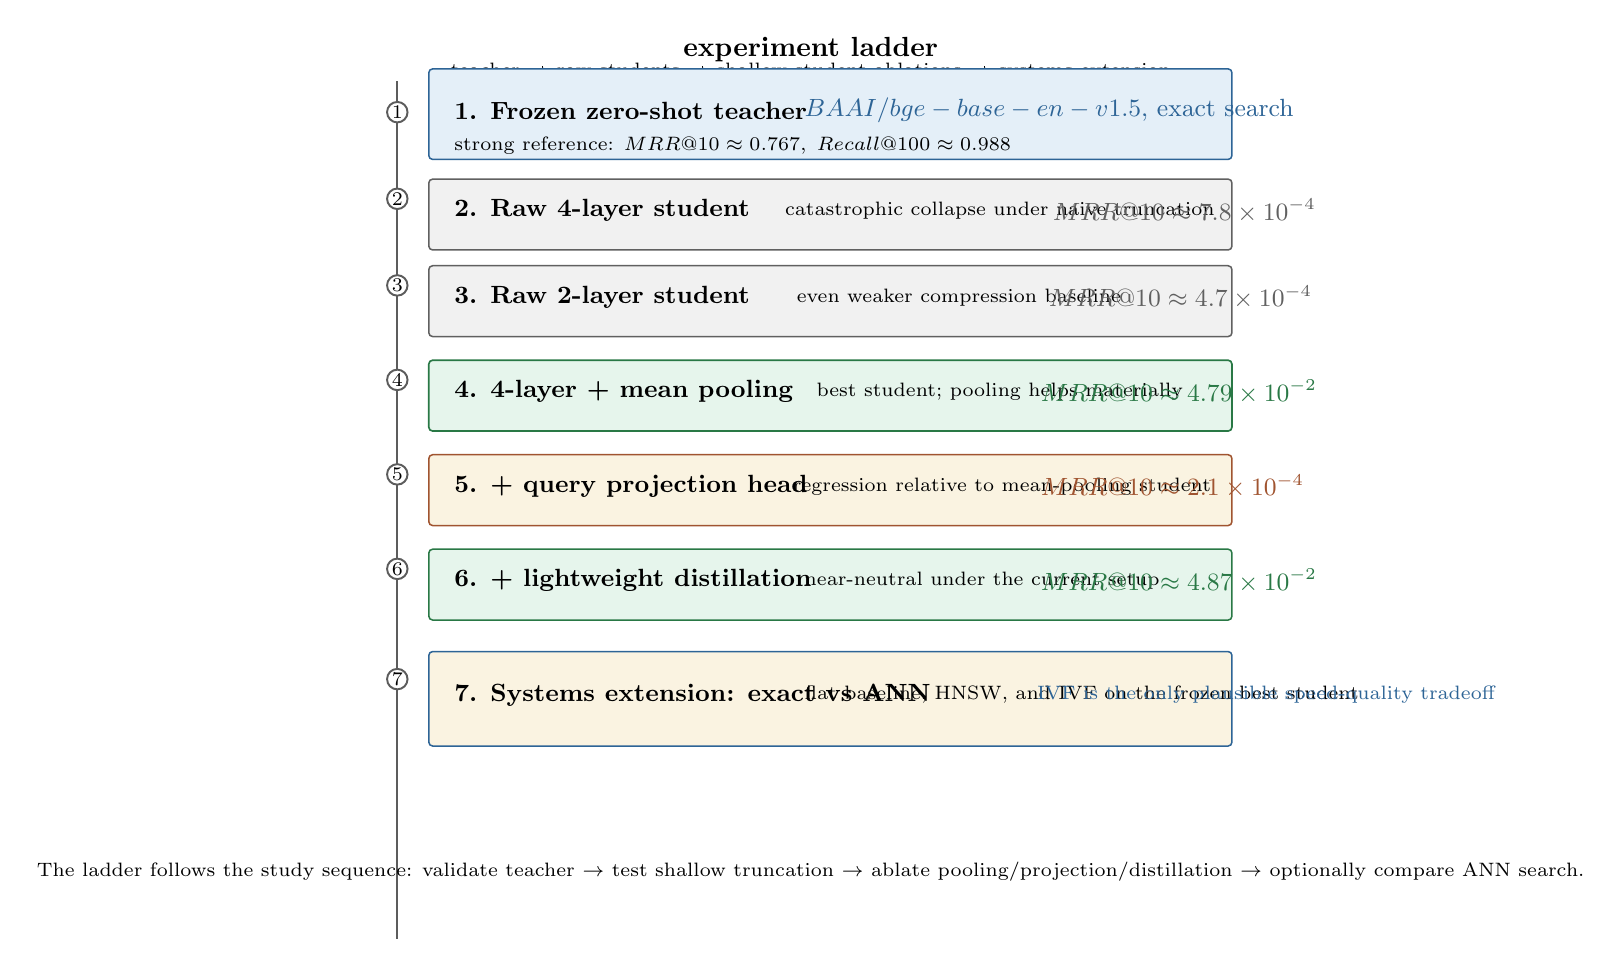
\begin{tikzpicture}[x=1cm,y=1cm, font=\small]
  \definecolor{stageblue}{RGB}{228,239,248}
  \definecolor{stagegray}{RGB}{241,241,241}
  \definecolor{stagegreen}{RGB}{230,245,236}
  \definecolor{stagered}{RGB}{250,233,233}
  \definecolor{stageamber}{RGB}{250,243,225}
  \definecolor{stepline}{RGB}{92,92,92}
  \definecolor{teacherline}{RGB}{45,100,150}
  \definecolor{studentline}{RGB}{96,96,96}
  \definecolor{bestline}{RGB}{41,120,69}
  \definecolor{warnline}{RGB}{160,84,48}

  % Vertical spine for the "ladder" metaphor.
  \draw[line width=0.7pt, draw=stepline] (0.95,0.7) -- (0.95,11.6);

  % Step markers.
  \foreach \yy/\lab in {11.2/1,10.1/2,9.0/3,7.8/4,6.6/5,5.4/6,4.0/7} {
    \fill[white] (0.95,\yy) circle (0.13);
    \draw[line width=0.7pt, draw=stepline] (0.95,\yy) circle (0.13);
    \node[font=\scriptsize] at (0.95,\yy) {\lab};
  }

  % Top annotation.
  \node[align=left, font=\bfseries] at (6.2,12.0) {experiment ladder};
  \node[align=left, font=\scriptsize] at (6.2,11.72) {teacher \textrightarrow\ raw students \textrightarrow\ shallow-student ablations \textrightarrow\ systems extension};

  % Step 1: teacher reference.
  \draw[rounded corners=1.4pt, line width=0.55pt, draw=teacherline, fill=stageblue] (1.35,10.6) rectangle (11.55,11.75);
  \node[anchor=west, align=left] at (1.55,11.22) {\textbf{1. Frozen zero-shot teacher}};
  \node[anchor=west, align=left, text=teacherline] at (6.0,11.22) {$\text{BAAI/bge-base-en-v1.5}$, exact search};
  \node[anchor=west, align=left] at (1.55,10.78) {\scriptsize strong reference: $MRR@10 \approx 0.767,\; Recall@100 \approx 0.988$};

  % Step 2: raw four-layer student.
  \draw[rounded corners=1.4pt, line width=0.55pt, draw=studentline, fill=stagegray] (1.35,9.45) rectangle (11.55,10.35);
  \node[anchor=west, align=left] at (1.55,9.95) {\textbf{2. Raw 4-layer student}};
  \node[anchor=west, align=left] at (5.75,9.95) {\scriptsize catastrophic collapse under naive truncation};
  \node[anchor=west, align=left, text=studentline] at (9.15,9.95) {$MRR@10 \approx 7.8\times10^{-4}$};

  % Step 3: raw two-layer student.
  \draw[rounded corners=1.4pt, line width=0.55pt, draw=studentline, fill=stagegray] (1.35,8.35) rectangle (11.55,9.25);
  \node[anchor=west, align=left] at (1.55,8.85) {\textbf{3. Raw 2-layer student}};
  \node[anchor=west, align=left] at (5.9,8.85) {\scriptsize even weaker compression baseline};
  \node[anchor=west, align=left, text=studentline] at (9.1,8.85) {$MRR@10 \approx 4.7\times10^{-4}$};

  % Step 4: best positive pooling ablation.
  \draw[rounded corners=1.4pt, line width=0.6pt, draw=bestline, fill=stagegreen] (1.35,7.15) rectangle (11.55,8.05);
  \node[anchor=west, align=left] at (1.55,7.65) {\textbf{4. 4-layer + mean pooling}};
  \node[anchor=west, align=left] at (6.15,7.65) {\scriptsize best student; pooling helps materially};
  \node[anchor=west, align=left, text=bestline] at (9.0,7.65) {$MRR@10 \approx 4.79\times10^{-2}$};

  % Step 5: projection head ablation.
  \draw[rounded corners=1.4pt, line width=0.55pt, draw=warnline, fill=stageamber] (1.35,5.95) rectangle (11.55,6.85);
  \node[anchor=west, align=left] at (1.55,6.45) {\textbf{5. + query projection head}};
  \node[anchor=west, align=left] at (5.85,6.45) {\scriptsize regression relative to mean-pooling student};
  \node[anchor=west, align=left, text=warnline] at (9.0,6.45) {$MRR@10 \approx 2.1\times10^{-4}$};

  % Step 6: lightweight distillation.
  \draw[rounded corners=1.4pt, line width=0.55pt, draw=bestline, fill=stagegreen] (1.35,4.75) rectangle (11.55,5.65);
  \node[anchor=west, align=left] at (1.55,5.25) {\textbf{6. + lightweight distillation}};
  \node[anchor=west, align=left] at (6.0,5.25) {\scriptsize near-neutral under the current setup};
  \node[anchor=west, align=left, text=bestline] at (9.0,5.25) {$MRR@10 \approx 4.87\times10^{-2}$};

  % Step 7: ANN extension.
  \draw[rounded corners=1.4pt, line width=0.55pt, draw=teacherline, fill=stageamber] (1.35,3.15) rectangle (11.55,4.35);
  \node[anchor=west, align=left] at (1.55,3.8) {\textbf{7. Systems extension: exact vs ANN}};
  \node[anchor=west, align=left] at (6.0,3.8) {\scriptsize flat baseline, HNSW, and IVF on the frozen best student};
  \node[anchor=west, align=left, text=teacherline] at (8.95,3.8) {\scriptsize IVF is the only plausible speed-quality tradeoff};

  % Footer annotation.
  \node[align=left, font=\scriptsize] at (6.2,1.55) {The ladder follows the study sequence: validate teacher $\rightarrow$ test shallow truncation $\rightarrow$ ablate pooling/projection/distillation $\rightarrow$ optionally compare ANN search.};
\end{tikzpicture}
